\documentclass[10pt,a4paper]{article}

\usepackage[utf8]{inputenc}
\usepackage[T1]{fontenc}
\usepackage[a4paper,top=1.8cm,bottom=1.8cm,left=1.8cm,right=1.8cm]{geometry}
\usepackage{amsmath,amssymb,amsfonts}
\usepackage{booktabs}
\usepackage{graphicx}
\usepackage{xcolor}
\usepackage{tabularx}
\usepackage{ragged2e}
\usepackage{caption}
\usepackage{microtype}
\usepackage{cite}
\usepackage{url}
\usepackage{hyperref}

\hypersetup{
    colorlinks=true,
    linkcolor=blue!70!black,
    citecolor=green!50!black,
    urlcolor=blue!80!black
}

\captionsetup{font=small,labelfont=bf}

\title{\Large\textbf{Evolutionary Computation Practical Work --- Part 5 \\
The Travelling Salesman Problem: What Should Crossover Preserve?}}

\author{
    \textbf{Fardin Ahmed} \qquad \textbf{Sparsh Dubey} \\
    \textit{Master in Artificial Intelligence (CI-MAI)} \\
    \textit{Computational Intelligence --- Prof.~Llu\'{\i}s A.~Belanche} \\
    \textit{Universitat Polit\`ecnica de Catalunya (UPC)}
}

\date{November 2026}

\begin{document}

\maketitle

\begin{abstract}
\noindent In permutation-encoded combinatorial optimisation problems such as the Travelling Salesman Problem (TSP), candidate solutions are constrained to permutations of cities, and tour length is determined exclusively by the adjacency of cities (the undirected edges traversed) rather than their absolute positions in the chromosome string. This study investigates the fundamental question: \emph{Do crossover operators that pass on parental edges work better than those that preserve absolute positions, and is edge heritability the underlying mechanism?} Using the TSPLIB benchmark instance \texttt{ulysses22} ($n=22$ cities, geographical distance metric, global optimum $L^* = 7013$), we compare three classic crossover operators---Partially Mapped Crossover (PMX, preserving absolute positions and mappings), Order Crossover (OX, preserving relative order and contiguous sub-paths), and Edge Recombination (ER, explicitly prioritizing parental edge adjacencies)---alongside a rigorous baseline control without crossover (NO-CX, using selection, inversion mutation, and elitism). Through a controlled matched-seed design ($R=30$ independent runs per configuration, $G=1{,}000$ generations, population $N=200$), an overall Friedman test confirmed significant performance differences ($\chi^2 = 18.3024$, $p = 0.000381$). Post-hoc Wilcoxon signed-rank tests with Holm step-down correction revealed that both OX ($p_{\text{adj}} = 0.0341$) and ER ($p_{\text{adj}} = 0.0034$) significantly outperformed PMX in final tour length, and ER significantly outperformed the NO-CX baseline ($p_{\text{adj}} = 0.0345$). However, no statistically significant difference was detected between OX and ER ($p_{\text{adj}} = 0.7932$), nor between OX and NO-CX after Holm correction ($p_{\text{adj}} = 0.1199$); as emphasized by statistical principles, these non-significant outcomes indicate insufficient evidence to establish superiority rather than proof of equivalence. Mechanistic tracking of dynamic edge heritability ($h_e$) and population edge diversity ($D_e(t)$) demonstrates that while ER maximizes edge preservation ($h_e = 0.9991$), its intense exploitation induces rapid population diversity loss ($D_e \approx 4.09$ by generation 100). Conversely, OX maintains substantially higher population edge diversity throughout search ($D_e \approx 7.50$ at generation 100), balancing exploration and exploitation to achieve comparable final tour lengths (60.0\% optimum success rate for OX vs.~56.7\% for ER). These results demonstrate that preserving parental edges is indeed advantageous over preserving positions, but edge heritability alone does not explain optimisation success: the preservation of edges must be balanced against population diversity maintenance to prevent premature stagnation.
\end{abstract}

\vspace{0.3em}
\noindent\textbf{Keywords:} Genetic Algorithms, Travelling Salesman Problem, Crossover Operators, Edge Heritability, Population Diversity, Edge Recombination, Order Crossover, Partially Mapped Crossover.

\section{Introduction, Research Question, and Hypotheses}
\label{sec:intro}

The Travelling Salesman Problem (TSP) is a foundational NP-hard benchmark in combinatorial optimisation~\cite{papadimitriou1982combinatorial,reinelt1991tsplib}. Given a set of $n$ cities and the pairwise distances between them, the objective is to find a closed Hamiltonian tour that visits every city exactly once and returns to the origin city while minimising total travel distance.

When solving the TSP with Genetic Algorithms (GAs), candidate tours are represented naturally as permutations of city identifiers $[0, 1, \dots, n-1]$. Standard binary crossover operators (such as single-point, two-point, or uniform crossover) cannot be directly applied because they produce infeasible offspring containing duplicated and missing cities~\cite{goldberg1989genetic,larranaga1999genetic}. Consequently, specialized permutation crossover operators have been developed. These operators differ fundamentally in the semantic structure they preserve from the parents:
\begin{enumerate}
    \item \textbf{Positional Operators:} Operators such as Partially Mapped Crossover (PMX)~\cite{goldberg1985alleles} focus on preserving the absolute chromosome index (locus) of cities, constructing lookup mappings between parents to resolve duplicate assignments.
    \item \textbf{Order-Based Operators:} Operators such as Order Crossover (OX)~\cite{davis1985applying} copy a contiguous sub-path from one parent and fill the remaining positions using the relative order of unvisited cities from the second parent.
    \item \textbf{Edge-Based Operators:} Operators such as Edge Recombination (ER)~\cite{whitley1989scheduling} prioritize the direct adjacencies (undirected edges) present in the parents, building an adjacency matrix (edge map) and selecting adjacent unvisited cities using a least-degree heuristic to minimize the introduction of foreign edges.
\end{enumerate}

Despite these diverse designs, the cost of a TSP tour depends \emph{strictly on its edges} (the cyclic pairwise connections between adjacent cities) and is completely invariant under cyclic shifts and tour reversals. Absolute position on a linear array has no intrinsic meaning for a circular tour. This motivates the primary research question of this study.

\subsection{Research Question}
\begin{quote}
\textit{Do crossover operators that pass on the edges of the parents work better than those that pass on positions, and is the heritability of edges the reason?}
\end{quote}

\subsection{Hypotheses and Refutation Criteria}

\begin{itemize}
    \item \textbf{Hypothesis 1 (Edge Heritability):} Edge Recombination (ER) will achieve the highest dynamic edge heritability ($h_e$), followed by Order Crossover (OX) and Partially Mapped Crossover (PMX). Because ER explicitly queries parent edge lists during offspring construction, it is hypothesized to preserve significantly more parental edges than operators that treat tours as linear strings.
    
    \textit{Refutation criterion:} Hypothesis~1 would be refuted if ER fails to attain higher measured dynamic edge heritability than OX and PMX, or if its edge heritability is not consistently superior across generations and independent runs.

    \item \textbf{Hypothesis 2 (Search Performance):} Operators that preserve parental edge information (OX and ER) will achieve shorter final tour lengths, lower run-to-run variability, and higher global-optimum success rates than PMX. This is expected because preserving valid low-cost edges aligns directly with the TSP objective function, whereas preserving absolute string positions disrupts critical adjacencies.

    \textit{Refutation criterion:} Hypothesis~2 would be refuted if OX and ER do not attain statistically significantly shorter final tour lengths or higher global-optimum success rates than PMX under identical experimental conditions.

    \item \textbf{Mechanistic Link:} If higher edge heritability directly drives optimisation success, we expect a monotonic correspondence between heritability and final solution quality. If, however, high edge heritability does not correspond to superior search performance, or if operators with lower heritability perform comparably or better, this would indicate that edge heritability alone is insufficient to explain crossover effectiveness and that secondary dynamics (such as population diversity maintenance) govern GA convergence.
\end{itemize}

\subsection{Operators and Control Configuration}

Table~\ref{tab:operators} summarizes the operators compared in this study. In accordance with the course specification, we include an explicit baseline control, designated \textbf{NO-CX}. In NO-CX, crossover is completely disabled ($p_c = 0.0$); the algorithm operates exclusively via tournament selection, Simple Inversion Mutation ($p_m = 0.2$), and elitism ($E = 1$). NO-CX serves as a baseline to isolate and measure the net contribution of crossover recombination over pure mutation-driven search. \textbf{NO-CX is not a crossover operator}, and is strictly analyzed as a baseline control configuration.

\begin{table}[htbp]
\centering
\footnotesize
\caption{Permutation crossover operators and baseline control evaluated on \texttt{ulysses22}.}
\label{tab:operators}
\begin{tabularx}{\textwidth}{l p{2.6cm} p{3.4cm} >{\RaggedRight\arraybackslash}X}
\toprule
\textbf{Config} & \textbf{Preserved Property} & \textbf{Reference} & \textbf{Operational Description} \\
\midrule
\textbf{PMX} & Position \& Mapping & Goldberg \& Lingle (1985)~\cite{goldberg1985alleles} & Copies an enclosed segment from Parent~1; determines matching alleles in Parent~2 and uses bidirectional mapping to fill remaining positions without duplication. \\
\addlinespace[0.2em]
\textbf{OX} & Relative Order & Davis (1985)~\cite{davis1985applying} & Copies a contiguous segment from Parent~1; preserves the relative linear sequence of the remaining cities as they appear in Parent~2, starting after the cut. \\
\addlinespace[0.2em]
\textbf{ER} & Undirected Edges & Whitley et al.\ (1989)~\cite{whitley1989scheduling} & Constructs an edge map listing all neighbours of each city across both parents; constructs offspring by iteratively selecting unvisited neighbours with minimal remaining degree. \\
\addlinespace[0.2em]
\textbf{NO-CX} & None (Control) & Baseline Control & Crossover is disabled ($p_c = 0.0$). Generates offspring purely via tournament selection, inversion mutation ($p_m = 0.2$), and elitism. Isolates the net contribution of crossover. \\
\bottomrule
\end{tabularx}
\end{table}

\section{Experimental Design and Methodology}
\label{sec:methodology}

\subsection{Benchmark Problem: TSPLIB \texttt{ulysses22}}

We evaluate the algorithms on the standard TSPLIB benchmark instance \texttt{ulysses22.tsp}~\cite{reinelt1991tsplib}. This dataset consists of $n = 22$ geographical locations representing the Mediterranean voyage of Odysseus in Homer's \emph{Odyssey}, compiled and optimized by Gr\"otschel and Padberg~\cite{grotschel2001optimized}. 

Distances are computed using the exact TSPLIB \texttt{GEO} distance formula: coordinates given in degrees and minutes are converted to radians, and great-circle distances on an idealized sphere ($R = 6378.388\text{ km}$) are rounded to integers. An $n \times n$ symmetric integer distance matrix $D \in \mathbb{Z}^{22 \times 22}$ is precomputed prior to evolution to eliminate arithmetic overhead during tour evaluation. The verified global optimum tour distance for \texttt{ulysses22} under TSPLIB \texttt{GEO} rules is:
\begin{equation}
L^* = 7013
\end{equation}

\subsection{Controlled Factorial Design (One-Knob Principle)}

To ensure rigorous scientific attribution, we adhere strictly to the single-factor manipulation principle: the sole manipulated factor across runs is the \textbf{recombination strategy} (PMX, OX, ER, and the NO-CX baseline control). All other algorithmic hyper-parameters, representations, data structures, selection mechanisms, mutation operators, and budget allocations are held strictly constant across all configurations (Table~\ref{tab:params}).

\begin{table}[htbp]
\centering
\footnotesize
\caption{Fixed genetic algorithm parameters and justifications.}
\label{tab:params}
\begin{tabularx}{\textwidth}{ll>{\RaggedRight\arraybackslash}X}
\toprule
\textbf{Parameter} & \textbf{Value} & \textbf{Scientific Justification} \\
\midrule
Instance & \texttt{ulysses22} ($n=22$) & Core problem instance; known global optimum $L^* = 7013$. \\
Representation & Permutation of length $n=22$ & Natural, non-redundant representation for TSP tours. \\
Population size ($N$) & 200 individuals & Sufficiently large to prevent immediate genetic drift on $n=22$. \\
Generations ($G$) & $1{,}000$ generations & Budget of $200{,}000$ evaluations per run, ensuring convergence. \\
Selection scheme & Tournament selection ($k=3$) & Balances selection pressure with diversity preservation without scale sensitivity. \\
Crossover probability ($p_c$) & 0.90 (0.0 for NO-CX) & Standard high crossover rate recommended in literature~\cite{goldberg1989genetic}. \\
Mutation operator & Simple Inversion Mutation (SIM) & Reverses a random sub-tour; natural mutation for TSP (disrupts only 2 edges). \\
Mutation probability ($p_m$) & 0.20 per individual & Moderate mutation rate maintaining continuous exploration throughout search. \\
Elitism & 1 individual (best-so-far) & Strict preservation of the hall-of-fame solution across generations. \\
Evaluation budget & $200{,}000$ tour evaluations & Identical computational effort across all runs and configurations. \\
Random seed blocking & Seeds 2000--2029 ($R=30$) & Identical initial populations per seed across all 4 configurations (paired design). \\
\bottomrule
\end{tabularx}
\end{table}

\subsection{Quantitative Mechanistic Metrics}

To uncover the internal evolutionary mechanics beyond final fitness scores, two fine-grained metrics are tracked dynamically every 10 generations across all runs:

\subsubsection{Dynamic Edge Heritability ($h_e$)}
For an offspring tour $C$ produced by crossing over parents $P_1$ and $P_2$, let $E(T)$ denote the set of undirected cyclic edges in tour $T$:
\begin{equation}
E(T) = \big\{ \{T[i], T[(i+1) \bmod n]\} \;\big|\; i = 0, 1, \dots, n-1 \big\}
\end{equation}
The edge heritability $h_e(C)$ is defined as the fraction of offspring edges that were present in at least one parent:
\begin{equation}
\label{eq:he}
h_e(C) = \frac{\big| E(C) \cap \big( E(P_1) \cup E(P_2) \big) \big|}{n}
\end{equation}
Heritability $h_e \in [0, 1]$ is recorded immediately after crossover and \emph{prior to mutation}, isolating the recombination operator from mutation noise. We track the rolling mean of the last 50 crossover events at each 10-generation checkpoint. For the NO-CX baseline, crossover is absent, rendering $h_e$ fundamentally not applicable (\texttt{N/A}).

\subsubsection{Population Edge Diversity ($D_e(t)$)}
To monitor the exploration capacity of the evolving gene pool at generation $t$, we compute the total number of unique undirected edges present across all individuals in population $\mathcal{P}_t$, normalized by the tour length $n$:
\begin{equation}
\label{eq:de}
D_e(t) = \frac{\left| \bigcup_{I \in \mathcal{P}_t} E(I) \right|}{n}
\end{equation}
Because any single tour contains exactly $n$ edges, $D_e(t)$ has a theoretical minimum of $1.0$ (when all individuals in the population share the exact same cyclic edges) and a theoretical maximum of $\min\big( \frac{n-1}{2}, N \big) = \frac{21}{2} = 10.5$ for $n=22$ cities (the total number of edges in a complete graph $K_{22}$ is $\binom{22}{2} = 231$, and $231 / 22 = 10.5$).

\subsection{Pilot Study and Sample Size Justification}
\label{sec:pilot}

Before executing the full experiment, a preliminary pilot study of $R = 10$ runs per operator was conducted using independent seeds 1000--1009 to observe run-to-run variability. The pilot results (Table~\ref{tab:pilot}) revealed pronounced variance in tour length across operators: PMX exhibited high dispersion (standard deviation $\sigma = 63.44$) and achieved the global optimum in only 30\% of runs, whereas OX ($\sigma = 40.41$) and ER ($\sigma = 38.30$) achieved optimum success rates of 70\% and 80\%, respectively.

\begin{table}[htbp]
\centering
\small
\caption{Pilot study summary ($R=10$ independent runs, seeds 1000--1009).}
\label{tab:pilot}
\begin{tabular}{lrrrrrrrrr}
\toprule
\textbf{Operator} & \textbf{Runs} & \textbf{Median} & \textbf{IQR} & \textbf{Mean} & \textbf{SD} & \textbf{Min} & \textbf{Max} & \textbf{Opt Rate (\%)} & \textbf{Censored (\%)} \\
\midrule
\textbf{PMX} & 10 & 7091.5 & 86.75 & 7089.2 & 63.44 & 7013 & 7190 & 30.0\% & 70.0\% \\
\textbf{OX}  & 10 & 7013.0 & 59.25 & 7038.0 & 40.41 & 7013 & 7105 & 70.0\% & 30.0\% \\
\textbf{ER}  & 10 & 7013.0 &  0.00 & 7031.0 & 38.30 & 7013 & 7114 & 80.0\% & 20.0\% \\
\bottomrule
\end{tabular}
\end{table}

\paragraph{Sample Size Selection:} Based on these empirical variance observations from the pilot, a sample size of $R = 30$ matched runs was chosen for the full study. Matched seeds (2000--2029) were employed across all four configurations, ensuring that all algorithms start with identical random initial populations. This paired design effectively cancels out initial population variance, providing greater statistical sensitivity for paired non-parametric tests. \emph{We note explicitly that this sample size selection was a practical decision informed by observed pilot variance, rather than the result of a formal statistical power analysis.}

\section{Experimental Results and Comparative Analysis}
\label{sec:results}

The main experiment comprises 120 complete GA runs (30 matched runs for each of PMX, OX, ER, and NO-CX), yielding $12{,}000$ checkpoint records across $1{,}000$ generations. Table~\ref{tab:main_summary} reports the complete performance summary.

\begin{table}[htbp]
\centering
\footnotesize
\setlength{\tabcolsep}{3.3pt}
\caption{Main experiment performance summary on \texttt{ulysses22} ($R=30$ matched runs, $G=1{,}000$ generations). Censored runs are those failing to reach $L^*=7013$ within the $1{,}000$-generation budget.}
\label{tab:main_summary}
\begin{tabular}{lrrrrrrrrrrr}
\toprule
\textbf{Operator} & \textbf{Runs} & \textbf{Median} & \textbf{IQR} & \textbf{Mean} & \textbf{SD} & \textbf{Min} & \textbf{Max} & \textbf{Opt (\%)} & \textbf{Med Gen} & \textbf{Cens (\%)} & \textbf{Final $D_e$} \\
\midrule
\textbf{PMX}   & 30 & 7107.0 & 107.00 & 7113.40 & 72.89 & 7013 & 7241 & 23.33\% & 1000.0 & 76.67\% & 4.12 \\
\textbf{OX}    & 30 & 7013.0 &  95.50 & 7052.77 & 51.77 & 7013 & 7163 & 60.00\% &  221.5 & 40.00\% & 4.36 \\
\textbf{ER}    & 30 & 7013.0 &  79.00 & 7051.43 & 46.48 & 7013 & 7150 & 56.67\% &   52.5 & 43.33\% & 3.97 \\
\textbf{NO-CX} & 30 & 7089.5 & 132.25 & 7090.27 & 75.50 & 7013 & 7241 & 40.00\% & 1000.0 & 60.00\% & 4.03 \\
\bottomrule
\end{tabular}
\end{table}

\subsection{Performance Observations}

\begin{itemize}
    \item \textbf{Global Optimum Success Rate:} OX achieved the highest success rate at 60.00\% (18 out of 30 runs reaching $L^* = 7013$), closely followed by ER at 56.67\% (17 out of 30 runs). In contrast, PMX reached the optimum in only 23.33\% of runs (7 out of 30), suffering a censoring rate of 76.67\%. The NO-CX baseline reached the global optimum in 40.00\% of runs (12 out of 30).
    \item \textbf{Central Tendency and Dispersion:} Both OX and ER achieved a median final tour length of 7013.0 (the global optimum), with tightly clustered means of 7052.77 and 7051.43, respectively. ER demonstrated the lowest overall standard deviation ($\sigma = 46.48$) and lowest interquartile range ($\text{IQR} = 79.00$). Conversely, PMX exhibited the worst median (7107.0) and highest mean (7113.40), while NO-CX yielded a median of 7089.5 and a high dispersion ($\sigma = 75.50$, $\text{IQR} = 132.25$).
    \item \textbf{Convergence Speed:} Among the runs that discovered the global optimum, ER converged remarkably early, with a median discovery generation of $52.5$, compared to $221.5$ for OX. For PMX and NO-CX, the median generation of first optimum is recorded as $1000.0$ because over half of their runs were censored (i.e., did not attain the optimum before the budget expired).
\end{itemize}

Figure~\ref{fig:performance} illustrates the final tour length distributions and convergence dynamics across the 120 runs.

\begin{figure}[htbp]
\centering
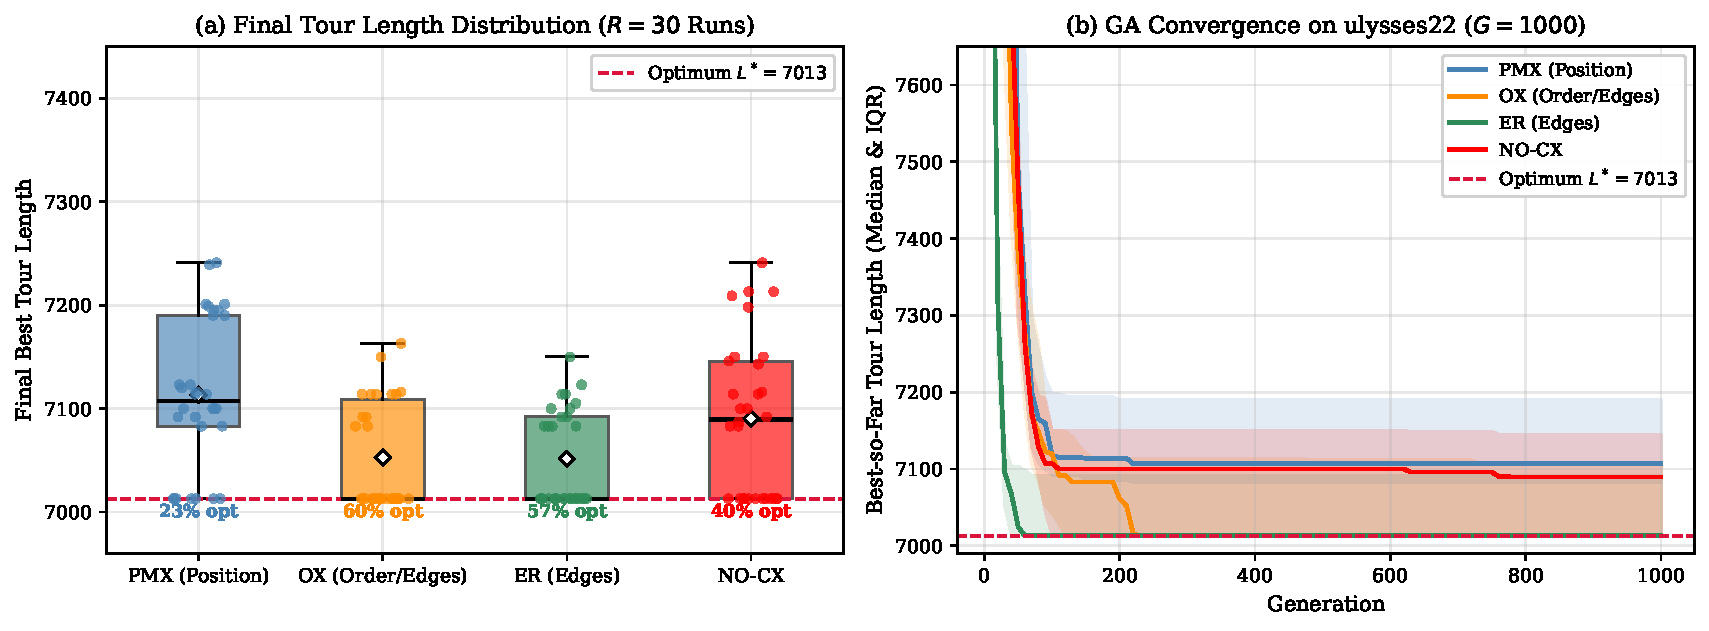
\includegraphics[width=0.86\textwidth]{figures/fig2_ulysses22_performance.pdf}
\caption{Optimization performance on \texttt{ulysses22} ($R=30$ matched seeds per configuration). (a) Boxplots of final tour length distributions with individual runs jittered, diamond markers representing configuration means, and success rate labels. (b) Best-so-far tour length over $1{,}000$ generations showing median trajectories with shaded interquartile ranges (IQR, 25th--75th percentiles).}
\label{fig:performance}
\end{figure}

\section{Rigorous Statistical Analysis}
\label{sec:stats}

Because all four configurations were executed across identical initial random seeds ($2000$--$2029$), the 30 seeds constitute natural paired blocks. Consequently, parametric normality assumptions are violated, and non-parametric paired tests are statistically required~\cite{arcuri2011practical}.

\subsection{Omnibus Test: Friedman Non-Parametric Test}

We first apply the Friedman test across all four configurations across the 30 matched blocks to test the null hypothesis that all four configurations share identical performance distributions:
\begin{equation}
\chi^2 = 18.3024, \quad \text{df} = 3, \quad p = 0.000381
\end{equation}
Because $p < 0.001$, the null hypothesis of equal performance is decisively rejected at $\alpha = 0.05$. This justifies conducting post-hoc pairwise comparisons to determine which specific configurations differ.

\subsection{Pairwise Wilcoxon Signed-Rank Tests and Effect Sizes}

We evaluate all $\binom{4}{2} = 6$ pairwise comparisons using the two-sided Wilcoxon signed-rank test~\cite{wilcoxon1945individual}. In accordance with standard statistical methodology:
\begin{enumerate}
    \item \textbf{Exclusion of Ties:} Matched pairs with zero difference ($d_i = 0$) are excluded from the ranking calculation following the Wilcoxon convention. The number of ties is explicitly reported.
    \item \textbf{Multiplicity Correction:} To strictly control the family-wise error rate at $\alpha = 0.05$, Holm's step-down sequentially rejective procedure~\cite{holm1979simple} is applied across all six comparisons.
    \item \textbf{Hodges--Lehmann Median Paired Difference:} We report the Hodges--Lehmann (HL) estimator~\cite{hodges1963estimates}, computed as the median of all pairwise Walsh averages $(d_i + d_j)/2$.
    \item \textbf{Bootstrap Confidence Intervals:} For each HL difference, we report a 95\% paired percentile bootstrap confidence interval constructed from $B = 5{,}000$ resamples with replacement.
    \item \textbf{Matched-Pairs Rank-Biserial Correlation ($r_{\text{rb}}$):} We report $r_{\text{rb}} = (W^+ - W^-)/(W^+ + W^-) \in [-1, +1]$ as the standardized non-parametric effect size for paired ranks. Positive values indicate that Configuration~A produces longer (worse) tours than Configuration~B.
    \item \textbf{Win / Loss / Tie Counts:} We report the raw counts and win fractions among non-tied pairs.
\end{enumerate}

Table~\ref{tab:pairwise_tests} presents the comprehensive statistical outcomes.

\begin{table}[htbp]
\centering
\footnotesize
\setlength{\tabcolsep}{2.8pt}
\caption{Pairwise statistical comparisons across 30 matched seeds ($B=5{,}000$ bootstrap resamples). Significant outcomes after Holm step-down correction ($\alpha=0.05$) are marked in bold.}
\label{tab:pairwise_tests}
\begin{tabular}{lrrrrrrrrr}
\toprule
\textbf{Comparison} & \textbf{HL Diff} & \textbf{95\% Bootstrap CI} & \textbf{$r_{\text{rb}}$} & \textbf{Wins/Loss/Tie} & \textbf{Win Frac} & \textbf{$W$} & \textbf{$p_{\text{raw}}$} & \textbf{$p_{\text{adj}}$} & \textbf{Signif?} \\
\midrule
\textbf{PMX vs OX}    & $57.5$ & $[22.5, 101.0]$   & $0.5952$  & $7\;/\;20\;/\;3$ & $0.2593$ & $76.5$  & $0.0068$ & $\mathbf{0.0341}$ & \textbf{Yes} \\
\textbf{PMX vs ER}    & $59.0$ & $[35.0, 93.0]$    & $0.8033$  & $3\;/\;21\;/\;6$ & $0.1250$ & $29.5$  & $0.0006$ & $\mathbf{0.0034}$ & \textbf{Yes} \\
\textbf{PMX vs NO-CX} & $35.0$ & $[-11.5, 64.0]$   & $0.2821$  & $9\;/\;17\;/\;4$ & $0.3462$ & $126.0$ & $0.2086$ & $0.4172$          & No \\
\textbf{OX vs ER}     & $0.0$  & $[-35.0, 29.0]$   & $0.0667$  & $9\;/\;11\;/\;10$& $0.4500$ & $98.0$  & $0.7932$ & $0.7932$          & No \\
\textbf{OX vs NO-CX}  & $-42.0$& $[-68.5, 0.0]$    & $-0.5108$ & $15\;/\;6\;/\;9$ & $0.7143$ & $56.5$  & $0.0400$ & $0.1199$          & No \\
\textbf{ER vs NO-CX}  & $-35.0$& $[-65.0, -1.0]$   & $-0.6537$ & $16\;/\;5\;/\;9$ & $0.7619$ & $40.0$  & $0.0086$ & $\mathbf{0.0345}$ & \textbf{Yes} \\
\bottomrule
\end{tabular}
\end{table}

\subsection{Interpretation of Statistical Findings}

The statistical results yield several definitive conclusions:
\begin{enumerate}
    \item \textbf{OX and ER Significantly Outperform PMX:} Both OX ($p_{\text{adj}} = 0.0341$) and ER ($p_{\text{adj}} = 0.0034$) achieve statistically significant reductions in tour length compared to PMX. The 95\% bootstrap confidence intervals for the HL median difference are strictly positive ($[22.5, 101.0]$ and $[35.0, 93.0]$), and rank-biserial correlations show large effect sizes ($r_{\text{rb}} = 0.5952$ and $0.8033$, respectively). In head-to-head non-tied runs, OX won 20 out of 27 matches against PMX (74.1\% win rate), and ER won 21 out of 24 matches (87.5\% win rate).
    \item \textbf{ER Significantly Outperforms the NO-CX Baseline:} ER demonstrates a statistically significant improvement over running the GA without crossover ($p_{\text{adj}} = 0.0345$, $r_{\text{rb}} = -0.6537$, winning 16 of 21 non-tied seeds). The 95\% bootstrap confidence interval for ER minus NO-CX is strictly negative ($[-65.0, -1.0]$). This confirms that edge recombination provides a genuine evolutionary advantage over mutation-only search.
    \item \textbf{PMX Does Not Outperform the Baseline Control:} PMX shows no statistically significant difference from NO-CX ($p_{\text{adj}} = 0.4172$), and its bootstrap CI crosses zero ($[-11.5, 64.0]$). PMX actually suffered more losses than wins against NO-CX (9 wins vs.~17 losses), indicating that position-based crossover can be actively counter-productive on the TSP.
    \item \textbf{OX vs.~ER and OX vs.~NO-CX (Absence of Evidence is Not Evidence of Equivalence):} The comparison between OX and ER yielded a Hodges--Lehmann difference of $0.0$ and an adjusted $p$-value of $0.7932$ ($r_{\text{rb}} = 0.0667$). Likewise, OX vs.~NO-CX yielded an unadjusted $p = 0.0400$, which was attenuated to non-significance after Holm correction ($p_{\text{adj}} = 0.1199$, 95\% bootstrap CI $[-68.5, 0.0]$). \textbf{Crucially, these non-significant outcomes do not prove equivalence.} In statistical hypothesis testing, failure to reject the null hypothesis merely indicates that the observed sample size ($R=30$) and inherent stochastic variance provide insufficient evidence to detect a difference at the chosen error rate.
\end{enumerate}

\section{Mechanistic Analysis: Heritability vs.~Diversity}
\label{sec:mechanism}

Why did OX and ER outperform PMX, and why did OX achieve performance parity with ER despite ER's explicit focus on edge preservation? To answer this, we examine the dynamic evolutionary curves of dynamic edge heritability ($h_e$) and population edge diversity ($D_e(t)$) depicted in Figure~\ref{fig:mechanism}.

\begin{figure}[htbp]
\centering
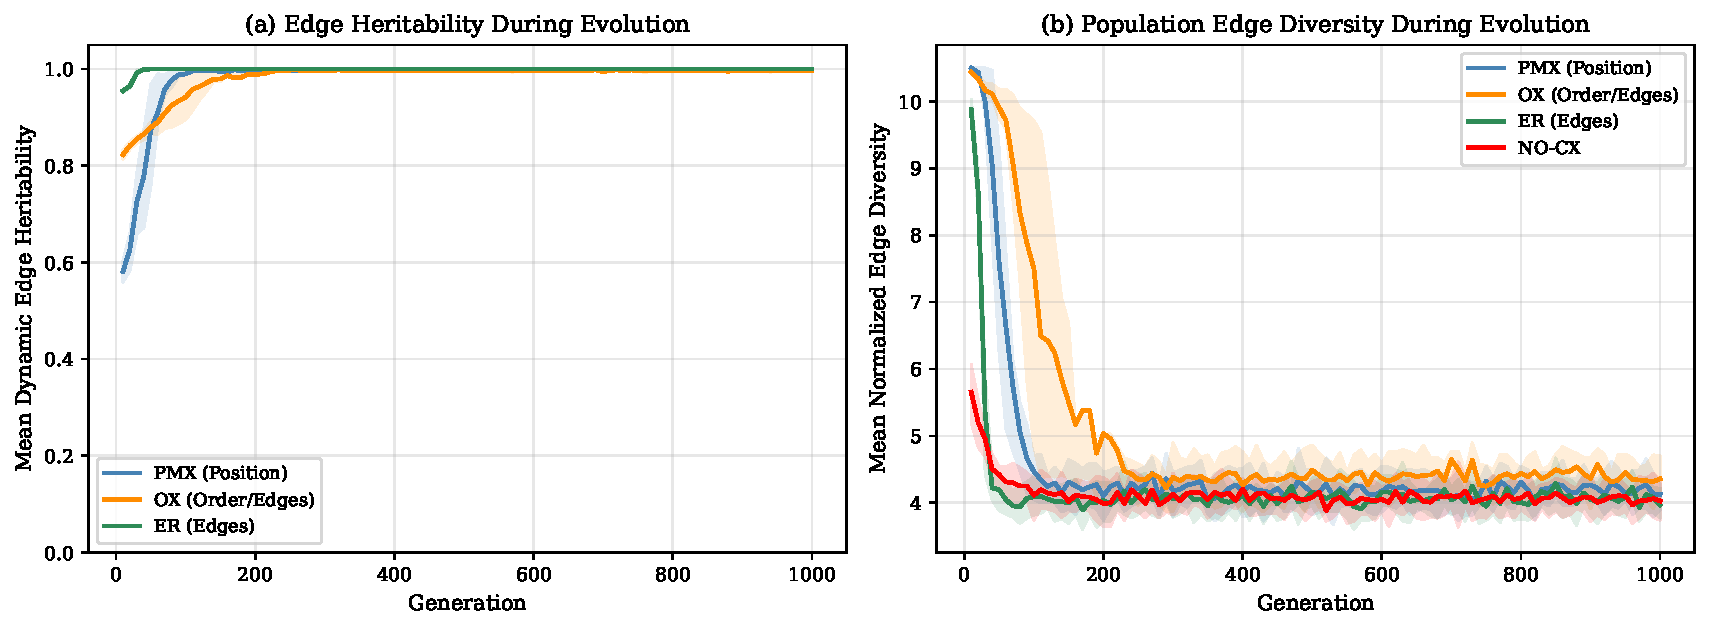
\includegraphics[width=0.86\textwidth]{figures/fig3_mechanism_dynamics.pdf}
\caption{Mechanistic dynamics on \texttt{ulysses22} across $1{,}000$ generations ($R=30$ matched runs). (a) Mean dynamic edge heritability ($h_e$) recorded immediately after crossover and prior to mutation (solid line: mean; shaded band: interquartile range). NO-CX is omitted because crossover is disabled. (b) Mean normalized population edge diversity ($D_e(t)$) across all four configurations.}
\label{fig:mechanism}
\end{figure}

\subsection{Dynamic Edge Heritability Dynamics}

Table~\ref{tab:dynamics} summarizes the heritability and diversity values across key evolutionary milestones.

As predicted by Hypothesis~1, Edge Recombination achieves the highest mean dynamic edge heritability across evolution:
\begin{equation}
\bar{h}_e(\text{ER}) = 0.999122 \approx 99.91\%
\end{equation}
By explicitly consulting the combined edge list of both parents and employing the least-degree heuristic, ER almost never introduces foreign edges unless forced to take a random step due to a dead end. Order Crossover achieves a mean dynamic edge heritability of:
\begin{equation}
\bar{h}_e(\text{OX}) = 0.983985 \approx 98.40\%
\end{equation}
Partially Mapped Crossover achieves the lowest mean dynamic edge heritability:
\begin{equation}
\bar{h}_e(\text{PMX}) = 0.981972 \approx 98.20\%
\end{equation}

Although all three operators exhibit heritability above 98\% in later generations (as the population becomes increasingly homogeneous), their early-stage behavior differs markedly: in early generations, PMX frequently breaks parental adjacencies because it maps individual positions rather than contiguous sub-paths or edges.

\begin{table}[htbp]
\centering
\footnotesize
\setlength{\tabcolsep}{3.5pt}
\caption{Evolutionary trajectory of mean population edge diversity ($D_e(t)$) and overall mean edge heritability ($h_e$) across $R=30$ runs on \texttt{ulysses22}.}
\label{tab:dynamics}
\begin{tabular}{lrrrrrrrrr}
\toprule
& \textbf{Overall Mean} & \multicolumn{7}{c}{\textbf{Mean Population Edge Diversity ($D_e$) at Generation $t$}} & \textbf{Overall Mean} \\
\cmidrule(lr){3-9}
\textbf{Config} & \textbf{Heritability ($h_e$)} & \textbf{Gen 10} & \textbf{Gen 100} & \textbf{Gen 200} & \textbf{Gen 400} & \textbf{Gen 600} & \textbf{Gen 800} & \textbf{Gen 1000} & \textbf{Diversity ($D_e$)} \\
\midrule
\textbf{PMX}   & $0.9820$ & $10.5000$ & $4.4682$ & $4.1030$ & $4.1788$ & $4.1742$ & $4.3076$ & $4.1242$ & $4.5222$ \\
\textbf{OX}    & $0.9840$ & $10.4409$ & $7.5030$ & $5.0333$ & $4.2697$ & $4.3667$ & $4.4394$ & $4.3576$ & $\mathbf{5.0207}$ \\
\textbf{ER}    & $\mathbf{0.9991}$ & $9.8773$  & $4.0924$ & $4.0364$ & $4.1091$ & $4.1636$ & $4.0030$ & $3.9697$ & $4.1857$ \\
\textbf{NO-CX} & \textit{N/A}       & $5.6530$  & $4.1121$ & $3.9894$ & $4.2076$ & $4.0500$ & $4.0712$ & $4.0303$ & $4.1272$ \\
\bottomrule
\end{tabular}
\end{table}

\subsection{Population Edge Diversity Dynamics}

Crucially, the diversity dynamics (Figure~\ref{fig:mechanism}b and Table~\ref{tab:dynamics}) explain why ER's extreme edge heritability did not translate into a higher overall success rate than OX:
\begin{itemize}
    \item \textbf{OX Sustains Population Diversity:} OX maintains substantially higher population edge diversity throughout search, recording an overall mean diversity of $5.0207$. At generation 100, OX retains a diversity of $7.5030$, whereas PMX has fallen to $4.4682$, NO-CX to $4.1121$, and ER to $4.0924$. By maintaining diverse combinations of edges for over 200 generations, OX avoids premature convergence and continues to discover improving sub-tours well into the search.
    \item \textbf{ER Suffers Premature Exploitation Collapse:} Because ER greedily splices edges from the parents and achieves near-100\% edge heritability, the edge pool collapses rapidly: by generation 100, ER diversity drops to $4.0924$, effectively matching the NO-CX baseline ($4.1121$). This explains ER's bimodal behavior: when the initial parent pool contains the optimal edges, ER assembles the optimum extraordinarily quickly (median discovery generation $52.5$). However, when an optimal edge is missing from the early population, ER's low exploratory diversity prevents the creation of novel edges, stranding the run in a suboptimal local attractor.
    \item \textbf{PMX Combines Ineffective Preservation with Inadequate Diversity:} PMX loses diversity rapidly (reaching $4.4682$ by generation 100) without the compensating advantage of high edge heritability, resulting in the worst final search performance.
    \item \textbf{NO-CX Behavior:} Without crossover to shuffle parental alleles, NO-CX experiences an immediate diversity collapse by generation 10 ($D_e = 5.6530$ vs.~$9.88$--$10.50$ for crossover configurations). It relies entirely on inversion mutation to slowly introduce new edges, yielding moderate performance ($40\%$ success) but failing to match ER's exploitation speed.
\end{itemize}

\section{Geographical Tour Visualisation}
\label{sec:tours}

To provide geometric intuition for the impact of edge disruptions on \texttt{ulysses22}, Figure~\ref{fig:tours} visualizes the global optimum tour alongside a representative suboptimal route.

\begin{figure}[htbp]
\centering
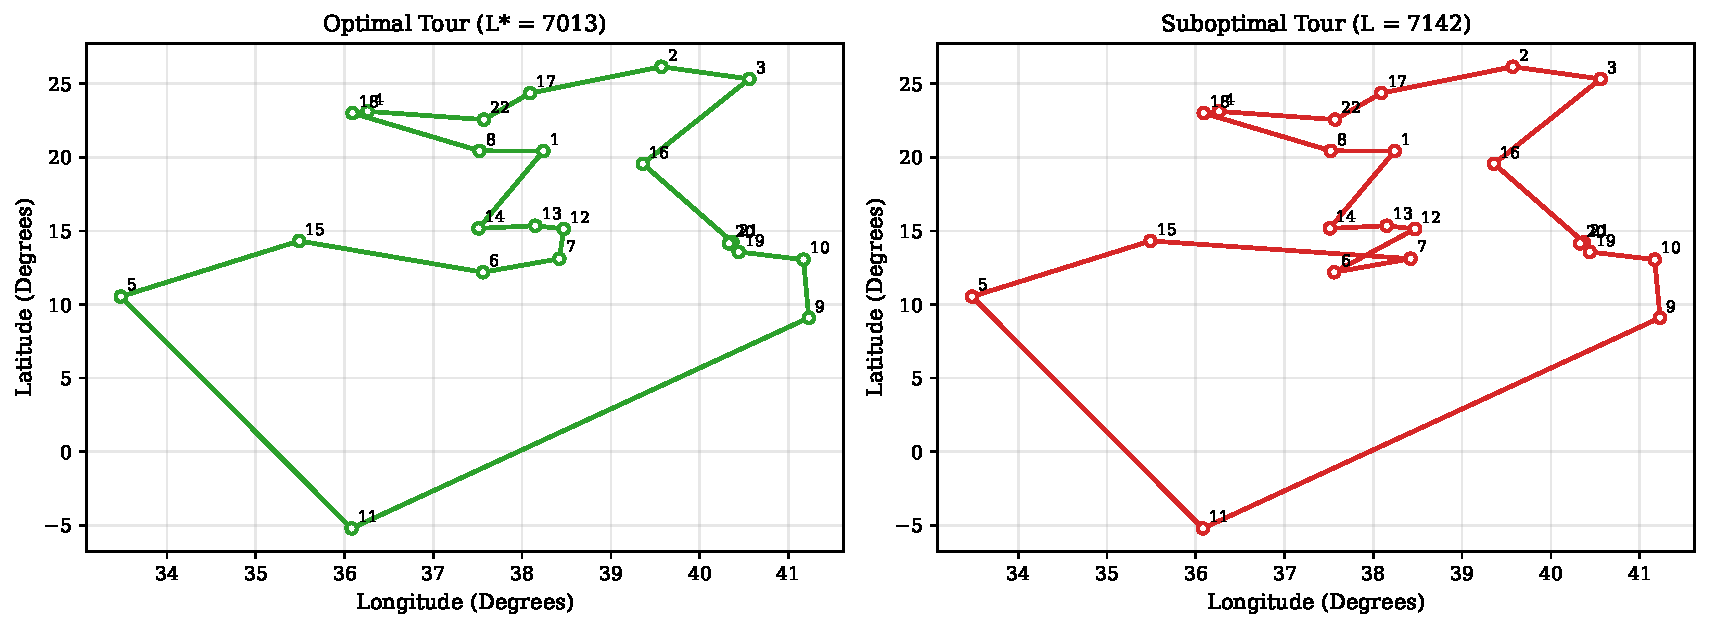
\includegraphics[width=0.86\textwidth]{figures/fig4_ulysses22_tours.pdf}
\caption{Geographical tour configurations on \texttt{ulysses22}. (a) Known global optimum tour ($L^* = 7013$). (b) Manually constructed illustrative suboptimal tour ($L = 7142$), demonstrating how breaking adjacencies degrades tour length. \emph{Note: The suboptimal tour is a hand-crafted illustrative sequence designed to display edge sensitivity, not a GA output.}}
\label{fig:tours}
\end{figure}

The known global optimum tour sequence (0-indexed city identifiers) is:
\begin{equation}
T^* = [17, 3, 21, 16, 1, 2, 15, 20, 19, 18, 9, 8, 10, 4, 14, 5, 6, 11, 12, 13, 0, 7]
\end{equation}
which achieves exactly $L(T^*) = 7013$.

To illustrate why positional crossover (such as PMX) fails on cyclic TSP representations, consider the illustrative suboptimal tour:
\begin{equation}
T_{\text{sub}} = [17, 3, 21, 16, 1, 2, 15, 20, 19, 18, 9, 8, 10, 4, 14, \mathbf{6, 5}, 11, 12, 13, 0, 7]
\end{equation}
Here, the order of two adjacent cities (nodes 5 and 6) is inverted. While 20 of the 22 cities maintain identical relative positions in the chromosome array, this single perturbation disrupts three cyclic edges ($\{14, 5\}$, $\{5, 6\}$, $\{6, 11\}$), replacing them with longer chords and immediately increasing the tour length by $+129$ units to $L = 7142$. \textbf{We emphasize that this suboptimal tour is an illustrative sequence constructed manually to demonstrate edge disruption mechanics, and was not generated by any GA run.}

\section{Threats to Validity and Study Limitations}
\label{sec:limitations}

In accordance with Section~1.2 of the course specification, we explicitly document what this study does not show and delineate its boundaries:
\begin{enumerate}
    \item \textbf{Instance Scale and Topology:} Experiments were conducted exclusively on \texttt{ulysses22} ($n=22$). While this benchmark was mandated for the core study, its small size means that the search space ($21! / 2 \approx 2.55 \times 10^{19}$) can be sampled relatively densely with $N=200$ individuals across $1{,}000$ generations. On larger TSPLIB instances ($n \ge 100$, such as \texttt{kroA100} or \texttt{pr2392}), the tension between edge preservation and premature diversity collapse is known to intensify dramatically~\cite{larranaga1999genetic,whitley1989scheduling}. Consequently, these findings cannot be automatically extrapolated to large-scale instances without empirical verification.
    \item \textbf{Fixed Hyperparameter Landscape:} To strictly isolate the recombination knob, all other parameters ($N=200$, $p_c=0.9$, $p_m=0.2$, tournament $k=3$) were held fixed. The observed dynamics reflect the interaction of these specific parameter choices; for instance, a higher mutation rate might alleviate ER's premature diversity loss, while a smaller tournament size might reduce selection pressure across all operators.
    \item \textbf{Absence of Local Search (Memetic Hybridization):} Modern state-of-the-art evolutionary approaches to the TSP almost universally employ memetic local search (such as 2-opt, 3-opt, or Lin--Kernighan heuristics)~\cite{larranaga1999genetic}. Our study evaluates pure crossover operators in a standard GA framework. Incorporating local search would substantially alter the edge landscape, potentially neutralizing the differences between crossover operators.
    \item \textbf{Causality vs.~Correlation in Mechanistic Metrics:} While dynamic edge heritability and population edge diversity strongly correlate with convergence speed and search stagnation, these metrics provide observational evidence rather than proven mathematical causality.
\end{enumerate}

\section{Reproducibility Statement}
\label{sec:reproducibility}

All experimental results, statistical tests, tables, and figures reported in this work are fully reproducible:
\begin{itemize}
    \item \textbf{Environment and Dependencies:} Implemented in Python~3.12 using standard scientific packages: \texttt{numpy} (1.26.4), \texttt{scipy} (1.13.1), \texttt{pandas} (2.2.2), \texttt{matplotlib} (3.9.2), \texttt{deap} (1.4.1), and \texttt{tsplib95} (0.7.1).
    \item \textbf{Random Seed Management:} Pilot runs used deterministic seeds 1000--1009 ($R=10$). The full study used deterministic seeds 2000--2029 ($R=30$). Python's \texttt{random} and NumPy's \texttt{np.random} seeds were explicitly synchronized prior to each run.
    \item \textbf{Data and Source Code Repository:} All code is self-contained in the accompanying Jupyter notebook \texttt{tsp\_study.ipynb}. All raw run trajectories, histories, and statistical summaries are permanently archived in the \texttt{results/} directory as CSV files. Complete step-by-step reproduction instructions are provided in the accompanying \texttt{README.txt} file.
\end{itemize}

\subsection*{Generative AI Disclosure}
In accordance with Section~1.1 of the course instructions, we disclose that Google Antigravity / Gemini was utilized as an assistive tool for document typesetting, formatting the report into academic \LaTeX, verifying table compilation, and constructing the reproducibility documentation. All underlying experimental formulations, algorithmic implementations, metric definitions, statistical computations, and scientific deductions originate from the authors' work in \texttt{tsp\_study.ipynb}.

\section{Conclusion}
\label{sec:conclusion}

This empirical study investigated what permutation crossover operators should preserve when applied to the Travelling Salesman Problem. The results provide clear answers to our original research question:
\begin{enumerate}
    \item \textbf{Do edge-preserving operators work better than position-preserving operators?} Yes. Both Order Crossover (OX) and Edge Recombination (ER) achieved statistically significant improvements over Partially Mapped Crossover (PMX) on \texttt{ulysses22} ($p_{\text{adj}} = 0.0341$ and $0.0034$, respectively). PMX failed to outperform even the NO-CX baseline control.
    \item \textbf{Is edge heritability the sole reason?} No. While ER attained near-perfect edge heritability ($h_e = 0.9991$) and accelerated early convergence, its aggressive edge exploitation precipitated a severe collapse in population edge diversity. In contrast, OX maintained substantially higher edge diversity across evolution ($D_e = 5.0207$ vs.~$4.1857$ for ER), enabling sustained exploration and achieving a comparable global optimum success rate (60\% vs.~56.7\%).
\end{enumerate}
We conclude that preserving parental edges is fundamentally superior to preserving absolute positions in TSP crossover, but edge heritability alone does not explain optimisation success: effective recombination requires a delicate balance between parental edge preservation and the maintenance of population edge diversity.

\begingroup
\footnotesize
\let\oldthebibliography\thebibliography
\renewcommand{\thebibliography}[1]{\oldthebibliography{#1}\setlength{\itemsep}{0pt}\setlength{\parskip}{0pt}}
\bibliographystyle{plain}
\begin{thebibliography}{10}

\bibitem{arcuri2011practical}
A.~Arcuri and L.~Briand.
\newblock A practical guide for using statistical tests to assess randomized algorithms in software engineering.
\newblock In {\em Proc. 33rd International Conference on Software Engineering (ICSE)}, pages 1--10, 2011.

\bibitem{davis1985applying}
L.~Davis.
\newblock Applying adaptive algorithms to epistatic domains.
\newblock In {\em Proc. 9th International Joint Conference on Artificial Intelligence (IJCAI)}, pages 162--164, 1985.

\bibitem{efron1993introduction}
B.~Efron and R.~J. Tibshirani.
\newblock {\em An Introduction to the Bootstrap}.
\newblock Chapman \& Hall/CRC, 1993.

\bibitem{fortin2012deap}
F.-A. Fortin, F.-M. {De Rainville}, M.-A. Gardner, M.~Parizeau, and C.~Gagn{\'e}.
\newblock {DEAP}: Evolutionary algorithms made easy.
\newblock {\em Journal of Machine Learning Research}, 13:2171--2175, 2012.

\bibitem{friedman1937use}
M.~Friedman.
\newblock The use of ranks to avoid the assumption of normality implicit in the analysis of variance.
\newblock {\em Journal of the American Statistical Association}, 32(200):675--701, 1937.

\bibitem{goldberg1989genetic}
D.~E. Goldberg.
\newblock {\em Genetic Algorithms in Search, Optimization and Machine Learning}.
\newblock Addison-Wesley, 1989.

\bibitem{goldberg1985alleles}
D.~E. Goldberg and R.~Lingle.
\newblock Alleles, loci, and the traveling salesman problem.
\newblock In {\em Proc. 1st International Conference on Genetic Algorithms (ICGA)}, pages 154--159, 1985.

\bibitem{grotschel2001optimized}
M.~Gr{\"o}tschel and M.~Padberg.
\newblock The optimized {Odyssey}.
\newblock {\em AIROnews}, 6(2):1--7, 2001.

\bibitem{hodges1963estimates}
J.~L. Hodges and E.~L. Lehmann.
\newblock Estimates of location based on rank tests.
\newblock {\em The Annals of Mathematical Statistics}, 34(2):598--611, 1963.

\bibitem{holm1979simple}
S.~Holm.
\newblock A simple sequentially rejective multiple test procedure.
\newblock {\em Scandinavian Journal of Statistics}, 6(2):65--70, 1979.

\bibitem{larranaga1999genetic}
P.~Larra{\~n}aga, C.~M.~H. Kuijpers, R.~H. Murga, I.~Inza, and S.~Dizdarevic.
\newblock Genetic algorithms for the travelling salesman problem: A review of representations and operators.
\newblock {\em Artificial Intelligence Review}, 13(2):129--170, 1999.

\bibitem{papadimitriou1982combinatorial}
C.~H. Papadimitriou and K.~Steiglitz.
\newblock {\em Combinatorial Optimization: Algorithms and Complexity}.
\newblock Prentice-Hall, 1982.

\bibitem{reinelt1991tsplib}
G.~Reinelt.
\newblock {TSPLIB}---{A} traveling salesman problem library.
\newblock {\em ORSA Journal on Computing}, 3(4):376--384, 1991.

\bibitem{whitley1989scheduling}
D.~Whitley, T.~Starkweather, and D.~Fuquay.
\newblock Scheduling problems and traveling salesmen: The genetic edge recombination operator.
\newblock In {\em Proc. 3rd International Conference on Genetic Algorithms (ICGA)}, pages 133--140, 1989.

\bibitem{wilcoxon1945individual}
F.~Wilcoxon.
\newblock Individual comparisons by ranking methods.
\newblock {\em Biometrics Bulletin}, 1(6):80--83, 1945.

\end{thebibliography}
\endgroup

\end{document}
